% 请确保在文档导言区(\documentclass 和 \begin{document} 之间)加载了 graphicx 宏包
% \usepackage{graphicx}

% --- 在你的 .tex 源文件中,把下面的 figure* 环境代码块 ---
% --- 放在 \section{Neural Radiance Fields (NeRF): Principles and Advancements} ---
% --- 这行的紧前面 ---
% --- 表格代码 (移除了 resizebox) ---

\begin{figure*}[t] % 使用 figure* 实现全宽效果,[t] 建议放在页面顶部
    \centering % 图像居中
    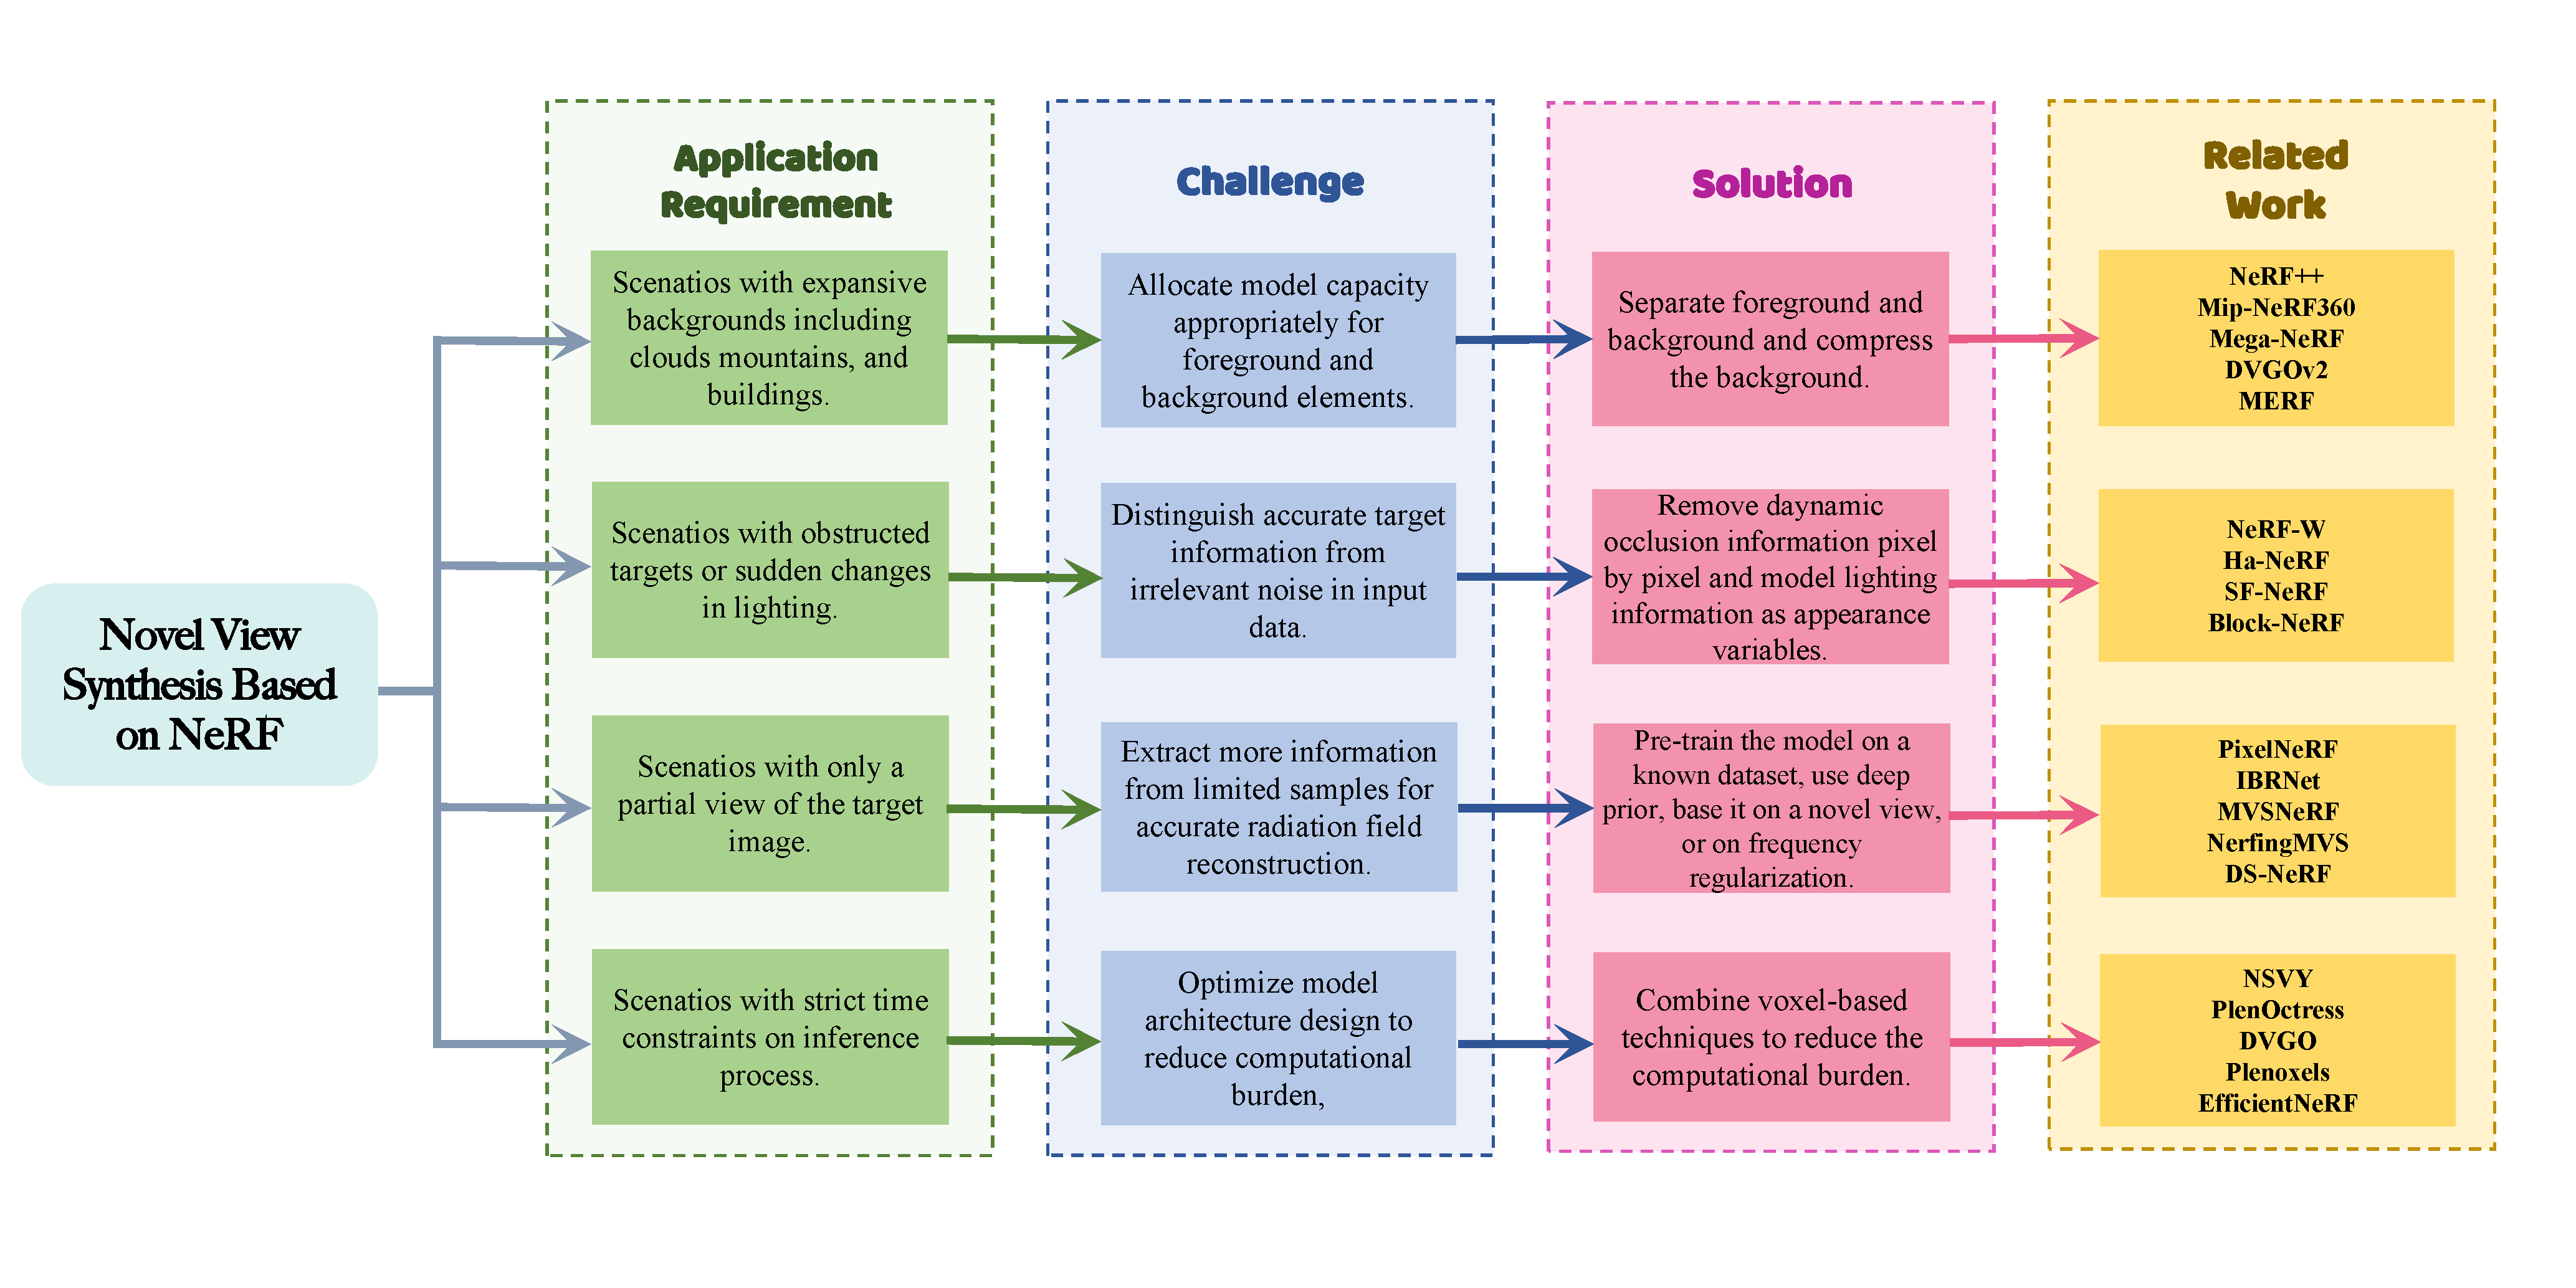
\includegraphics[
        width=\textwidth,        % 保持最终显示的宽度为文本宽度
        % --- 添加/修改裁切设置 ---
        trim={1cm 2cm 1cm 2cm}, % 【关键】设置裁切量:左(L) 下(B) 右(R) 上(T) - 请替换这些数值!
        clip                     % 【关键】应用裁切
        % --- 结束添加/修改 ---
    ]{./fig/NeRF.pdf}         % 你的 NeRF 图文件路径
    % 标题,可以注明是裁切后的视图
    \caption{Overview of NeRF-based Novel View Synthesis, illustrating the relationship between application requirements, key challenges, common solution strategies, and related works across different research directions. }
    % 建议使用不同的标签,标明是裁切版本
    \label{fig:nerf_challenges_summary}
\end{figure*}

%%%%%%%%%%%%%%%%%%%%%%%%%%%%%%%%%%%%%%%%%%%%%%%%%%%%%%%%%%%%%%%
% Main Body: Focusing on NeRF (Revised Version)
%%%%%%%%%%%%%%%%%%%%%%%%%%%%%%%%%%%%%%%%%%%%%%%%%%%%%%%%%%%%%%%

\section{Neural Radiance Fields (NeRF): Principles and Advancements}
\label{sec:nerf_main}

As introduced, the trajectory of Novel View Synthesis (NVS) took a sharp turn with the advent of Neural Radiance Fields (NeRF)~\cite{mildenhall2020nerf}. This method provided a powerful paradigm shift away from explicit geometric representations towards continuous, implicit scene modeling optimized via analysis-by-synthesis. Its ability to generate highly photorealistic and view-consistent results from captured images established it as a cornerstone technology, sparking extensive follow-up research aimed at addressing its initial limitations and broadening its applicability. This section first reviews the core principles of NeRF and then delves into the major advancements categorized by the key challenges encountered in real-world scenarios, referencing the overview presented in Figure~\ref{fig:nerf_challenges_summary}. % TODO: Update label if needed

\subsection{NeRF Core Principles}
\label{subsec:nerf_principles_revised}

NeRF represents a static scene as a continuous 5D function, typically implemented as a Multi-Layer Perceptron (MLP), $F_{\Theta}$. This function maps a 3D location $\mathbf{x}=(x,y,z)$ and a 2D viewing direction $\mathbf{d}=(\theta, \phi)$ to a volume density $\sigma$ and view-dependent RGB color $\mathbf{c}$~\cite{mildenhall2020nerf}:
\begin{equation}
    F_{\Theta}: (\mathbf{x}, \mathbf{d}) \rightarrow (\mathbf{c}, \sigma)
    \label{eq:nerf_func}
\end{equation}
To handle the fine geometric and appearance details, the 5D input coordinates $(\mathbf{x}, \mathbf{d})$ are first mapped to a higher-dimensional feature space using a positional encoding $\gamma(\cdot)$, which helps the MLP learn high-frequency functions~\cite{mildenhall2020nerf}.

Rendering involves casting camera rays $\mathbf{r}(t) = \mathbf{o} + t\mathbf{d}$ for each pixel, sampling points along these rays, querying the MLP $F_{\Theta}$ (using the positionally encoded inputs) to get $(\mathbf{c}, \sigma)$ at each sample point, and then approximating the volume rendering integral~\cite{kajiya1984ray, mildenhall2020nerf} to compute the final pixel color $\hat{C}(\mathbf{r})$. This is calculated via the discrete summation:
% --- 修改后的公式:将 T_i 的定义分开 ---
\begin{equation}
    \hat{C}(\mathbf{r}) = \sum_{i=1}^{N} T_i (1 - \exp(-\sigma_i \delta_i)) \mathbf{c}_i,
\label{eq:volume_rendering_discrete} % 主公式的标签
\end{equation}
where $T_i$ represents the accumulated transmittance along the ray up to sample $i$, defined as:
\begin{equation}
    T_i = \exp\left(-\sum_{j=1}^{i-1} \sigma_j \delta_j\right).
\label{eq:transmittance_discrete} % T_i 定义的标签 (如果需要单独引用)
\end{equation}
% --- 公式修改结束 ---
Here, $\sigma_i$ and $\mathbf{c}_i$ are the density and color of the $i$-th sample, and $\delta_i$ is the distance between adjacent samples. A hierarchical sampling strategy with "coarse" and "fine" networks is used to concentrate samples in relevant regions of space~\cite{mildenhall2020nerf}. The entire model $F_{\Theta}$ is optimized end-to-end by minimizing the photometric reconstruction loss between rendered pixel colors $\hat{C}(\mathbf{r})$ and ground truth pixel colors from input images.

An early, significant improvement was Mip-NeRF~\cite{barron2021mipnerf}, which addressed aliasing artifacts caused by NeRF's ray-point sampling at varying scales. By instead reasoning about conical frustums along rays and using integrated positional encodings, Mip-NeRF achieved better anti-aliasing and detail, becoming a strong baseline upon which many subsequent works were built.

Despite these foundational successes, applying NeRF effectively often requires overcoming specific hurdles related to scene properties, data capture conditions, and computational constraints.

\subsection{Challenge: Handling Unbounded Scenes}
\label{subsec:unbounded_challenge_revised}

\textbf{Problem:} Capturing scenes "in the wild" often involves vast, distant backgrounds (sky, landscapes) that extend effectively to infinity. Vanilla NeRF and Mip-NeRF, primarily designed for bounded object-centric scenes or forward-facing captures using coordinate normalization (NDC), struggle to represent these unbounded $360^\circ$ environments effectively, facing challenges in parameterization and efficient sampling~\cite{zhang2020nerfplusplus, barron2022mipnerf360}. Allocating model capacity appropriately between the near-field foreground and far-field background is crucial.

\textbf{Advancements:} A key solution involves parameterization techniques that map infinite exterior regions into a bounded domain. NeRF++~\cite{zhang2020nerfplusplus} pioneered a two-component approach, using standard coordinates inside a unit sphere for the foreground and an inverted sphere parameterization for the background, with separate MLPs for each. Mip-NeRF 360~\cite{barron2022mipnerf360} proposed an elegant scene contraction function based on squared distance that maps distant coordinates towards the surface of a sphere of radius 2, allowing a single Mip-NeRF model to represent the entire unbounded scene. It also introduced a distortion-based regularizer to encourage compact representations. This contraction technique became highly influential. Zip-NeRF~\cite{barron2023zipnerf}, for example, integrated this contraction with efficient grid-based representations (inspired by Instant NGP~\cite{mueller2022instant}) and improved sampling, achieving state-of-the-art quality and speed for unbounded scenes.

\subsection{Challenge: Modeling Dynamic Scenes and Appearance Variations}
\label{subsec:dynamic_challenge_revised}

\textbf{Problem:} Real-world data often violates NeRF's core assumption of a static scene. Transient elements like pedestrians or vehicles, as well as appearance changes due to variable lighting conditions, shadows, or camera auto-exposure, can lead to significant blurring, ghosting, or inconsistencies in the reconstruction~\cite{martinbrualla2021nerfw, tancik2022blocknerf}. Effectively distinguishing the underlying static scene from these dynamic factors is necessary.

\textbf{Advancements:} To address appearance variations and non-static elements, NeRF-W (NeRF in the Wild)~\cite{martinbrualla2021nerfw} introduced the idea of augmenting the NeRF architecture. It learns a per-image latent embedding vector to capture appearance variations (lighting, exposure) and adds a separate "transient" MLP branch that predicts color and density for dynamic objects, allowing the static branch to focus on the consistent scene structure. Block-NeRF~\cite{tancik2022blocknerf} scaled these ideas to city-scale scenes by decomposing the environment into individually trained NeRF blocks, each conditioned on appearance embeddings and time, while explicitly detecting and modeling transient objects (like vehicles) often using semantic segmentation priors.

\subsection{Challenge: Reconstruction from Few or Sparse Views}
\label{subsec:sparse_challenge_revised}

\textbf{Problem:} Optimizing NeRF typically requires dense image capture (dozens to hundreds of views) covering the scene well. When only a few input views are available (few-shot NVS), the reconstruction problem becomes severely ill-posed, often leading to overfitting, geometric inaccuracies, and unrealistic novel views~\cite{yu2021pixelnerf, niemeyer2022regnerf}. Extracting robust 3D information from limited samples is the core difficulty.

\textbf{Advancements:} Solutions broadly fall into two categories: incorporating learned priors or applying regularization.
(1) \textbf{Learned Priors:} Methods like PixelNeRF~\cite{yu2021pixelnerf} leverage large-scale pre-training on multi-view datasets. They use a CNN to extract image features from input views, which then condition the NeRF MLP prediction based on the projected sample point location, enabling generalization to new scenes from one or few views. MVSNeRF~\cite{chen2021mvsnerf} similarly uses pre-training but incorporates ideas from multi-view stereo by building a feature volume to guide the NeRF MLP.
(2) \textbf{Regularization/Optimization Strategies:} Other methods focus on adding regularization terms during NeRF optimization for the specific sparse scene, without requiring extensive pre-training. DietNeRF~\cite{jain2021dietnerf} encouraged semantic consistency between rendered novel views and input views using features from pre-trained vision-language models like CLIP. RegNeRF~\cite{niemeyer2022regnerf} introduced regularizers that promote geometric smoothness by penalizing inconsistencies in rendered depth patches across different views. FreeNeRF~\cite{yang2023freenerf} provided a simple yet effective frequency annealing strategy for the positional encoding, starting with low frequencies and gradually introducing higher ones, which significantly reduces overfitting in sparse settings.

\subsection{Challenge: Accelerating Training and Inference}
\label{subsec:acceleration_challenge_revised}

\textbf{Problem:} The need to query a potentially large MLP hundreds of times for every pixel ray makes both the training optimization and the rendering process computationally intensive and time-consuming (minutes to hours or days for training, seconds per frame for rendering)~\cite{mueller2022instant, chen2022tensorf}. This severely limits NeRF's use in interactive or real-time applications. Optimizing the architecture and query process is essential.

\textbf{Advancements:} A highly successful direction involves replacing the purely implicit MLP representation with hybrid approaches that leverage explicit data structures for faster querying. PlenOctrees~\cite{yu2021plenoctrees} demonstrated real-time rendering by pre-baking a trained NeRF into an octree storing density and spherical harmonic coefficients, though the baking process itself was slow. Subsequent works focused on *fast optimization* of these explicit structures. DVGO~\cite{sun2022dvgo} and Plenoxels~\cite{fridovichkeil2022plenoxels} directly optimized density and appearance features (like spherical harmonics) stored on voxel grids (dense or sparse), largely removing the need for MLPs and achieving training times in minutes. TensoRF~\cite{chen2022tensorf} proposed factorizing the 4D radiance field into compact tensor components (using techniques like CP or VM decomposition), significantly reducing memory footprint while enabling fast reconstruction. Perhaps most impactful was Instant NGP~\cite{mueller2022instant}, which introduced multi-resolution hash grid encodings. This technique uses hash tables to store feature vectors corresponding to different resolution levels, queried via interpolation, allowing a very small MLP to reconstruct high-frequency details rapidly. This enabled high-quality NeRF training in seconds to minutes on a single GPU.

\begin{table*}[t] % 使用 table* 横跨双栏,[t] 建议放顶部
    \centering
    \caption{Performance comparison of NeRF acceleration methods on the NeRF-Synthetic dataset. Metrics include PSNR↑ (higher is better), SSIM↑ (higher is better), LPIPS↓ (lower is better), Rendering Speed(FPS)↑ (higher is better), and Training Time↓ (lower is better). Data adapted from He et al.~\cite{He2024Progress}.}
    \label{tab:nerf_acceleration_comparison} % 表格标签
    % --- Resizebox 已被移除 ---
    \begin{tabular}{l c c c c c}
      \toprule
      Method & PSNR↑ & SSIM↑ & LPIPS↓ & Speed (FPS)↑ & Training Time↓ \\
      \midrule
      NeRF~\cite{mildenhall2020nerf}        & 31.01 & 0.947 & 0.081 & 0.023 & ~56 h \\
      NSVF~\cite{liu2020nsvf}               & 31.75 & 0.953 & 0.047 & 0.815 & ~100 h \\
      PlenOctrees~\cite{yu2021plenoctrees} & 31.71 & 0.958 & 0.053 & 167.68 & ~58 h (incl. baking) \\
      DVGO~\cite{sun2022dvgo}               & 31.95 & 0.957 & 0.053 & -     & ~14.2 min \\
      DVGOv2~\cite{sun2022dvgo}             & 32.76 & 0.962 & 0.046 & -     & ~6 min \\
      Plenoxels~\cite{fridovichkeil2022plenoxels} & 31.71 & 0.958 & 0.049 & -     & ~11 min \\
      ReLU Fields~\cite{karnewar2022relu}       & 30.04 & -     & 0.050 & -     & ~10 min \\
      TensoRF~\cite{chen2022tensorf}           & 33.14 & 0.963 & 0.047 & -     & ~17.6 min \\
      PlenVDB~\cite{yan2023plenvdb}             & 31.90 & -     & -     & 20.75 & ~12.4 min \\
      EfficientNeRF~\cite{hu2022efficientnerf} & 31.68 & 0.954 & 0.028 & 238.46 & ~6 h \\
      Instant NGP~\cite{mueller2022instant}   & 32.11 & 0.961 & 0.053 & -     & ~5 min \\
      NeRFAcc~\cite{li2023nerfacc}           & 33.11 & -     & 0.053 & -     & ~4.5 min \\
      \bottomrule
    \end{tabular}%
    % --- 对应的 resizebox 结束 } 已被移除 ---
  \end{table*}


\subsection{Summary and Outlook}
The advancements discussed highlight the rapid maturation of NeRF. By addressing challenges related to scene scale, dynamics, data sparsity, and computational cost, NeRF variants have become increasingly practical and versatile. Research continues to push boundaries, exploring further improvements in fidelity, speed, editability, and generalization, solidifying NeRF's role as a central pillar in modern 3D computer vision and graphics.

% TODO: Consider adding a concluding transition to the next section (e.g., Experiments) if applicable.

  


% --- 紧接着开始你的 NeRF 主体章节 ---


% %%%%%%%%%%%%%%%%%%%%%%%%%%%%%%%%%%%%%%%%%%%%%%%%%%%%%%%%%%%%%%%
% % Main Body: Focusing on NeRF
% %%%%%%%%%%%%%%%%%%%%%%%%%%%%%%%%%%%%%%%%%%%%%%%%%%%%%%%%%%%%%%%

% \section{Neural Radiance Fields (NeRF): Principles and Advancements}
% \label{sec:nerf_main}

% As highlighted in the introduction, Neural Radiance Fields (NeRF)~\cite{mildenhall2020nerf} represent a pivotal development in NVS, offering unprecedented photorealism by modeling scenes as continuous volumetric functions. This section delves into the core principles of NeRF and discusses the subsequent research avenues driven by practical application requirements and inherent challenges.

% \subsection{NeRF Core Principles}
% \label{subsec:nerf_principles}

% The fundamental idea behind NeRF~\cite{mildenhall2020nerf} is to represent a static scene using a fully-connected neural network (typically an MLP). This network, $F_{\Theta}$, maps a continuous 5D coordinate (3D location $\mathbf{x}=(x,y,z)$ and 2D viewing direction $\mathbf{d}=(\theta, \phi)$) to a volume density $\sigma$ and view-dependent emitted radiance (RGB color) $\mathbf{c}$.
% \begin{equation}
%     F_{\Theta}: (\mathbf{x}, \mathbf{d}) \rightarrow (\mathbf{c}, \sigma)
% \end{equation}
% To render a novel view, rays are cast from the virtual camera center through each pixel. Points are sampled along each ray $\mathbf{r}(t) = \mathbf{o} + t\mathbf{d}$. The color and density at these points are predicted by the MLP. The final pixel color $\hat{C}(\mathbf{r})$ is then computed by integrating the color and density along the ray using principles of volume rendering~\cite{kajiya1984ray, mildenhall2020nerf}:
% \begin{equation}
%     \hat{C}(\mathbf{r}) = \int_{t_n}^{t_f} T(t) \sigma(\mathbf{r}(t)) \mathbf{c}(\mathbf{r}(t), \mathbf{d}) dt,
%     \label{eq:volume_rendering_latex}
% \end{equation}
% where $t_n$ and $t_f$ are the near and far bounds, and $T(t) = \exp\left(-\int_{t_n}^{t} \sigma(\mathbf{r}(s)) ds\right)$ represents the accumulated transmittance, indicating the probability that the ray travels from $t_n$ to $t$ without being occluded~\cite{mildenhall2020nerf}. Hierarchical volume sampling is typically employed to efficiently sample relevant regions along the ray~\cite{mildenhall2020nerf}.

% % TODO: Briefly explain positional encoding and its importance for capturing high-frequency details. You could also add a sentence about Mip-NeRF~\cite{barron2021mipnerf} here as a common baseline improvement for anti-aliasing if desired.

% Despite its success, the original NeRF formulation encounters limitations in various real-world scenarios, motivating numerous subsequent extensions and improvements, often categorized by the specific challenge they address (as summarized in Figure~\ref{fig:nerf_challenges_summary} based on~\cite{NeRF_pdf_figure, He2024Progress}). % TODO: Update fig:nerf_challenges_summary to your actual figure label if you include the diagram.

% \subsection{Challenge: Handling Unbounded Scenes}
% \label{subsec:unbounded_challenge}

% \textbf{Problem:} Standard NeRF struggles with $360^\circ$ scenes containing very distant elements (e.g., sky), as its coordinate parameterization and sampling are typically designed for bounded volumes~\cite{zhang2020nerfplusplus, barron2022mipnerf360}. This aligns with the application requirement for scenarios with expansive backgrounds~\cite{NeRF_pdf_figure}. The core challenge is allocating model capacity effectively between foreground and background~\cite{NeRF_pdf_figure}.

% \textbf{Solutions:} A common strategy involves decomposing the scene representation~\cite{NeRF_pdf_figure}. NeRF++~\cite{zhang2020nerfplusplus} utilized separate MLPs for foreground and background regions, employing an inverted sphere parameterization for the latter. Mip-NeRF 360~\cite{barron2022mipnerf360} introduced a scene contraction technique combined with distortion regularization, becoming a standard for high-quality unbounded scene reconstruction. More recently, Zip-NeRF~\cite{barron2023zipnerf} built upon these ideas, integrating grid-based representations~\cite{mueller2022instant} for state-of-the-art results.

% % TODO: Add a sentence or two elaborating on the scene contraction technique in Mip-NeRF 360 or the decomposition in NeRF++.

% \subsection{Challenge: Modeling Dynamic Scenes and Appearance Variations}
% \label{subsec:dynamic_challenge}

% \textbf{Problem:} The static scene assumption of vanilla NeRF is violated in real-world captures containing transient objects (people, vehicles) or appearance changes due to varying illumination or camera settings, resulting in artifacts~\cite{martinbrualla2021nerfw, tancik2022blocknerf}. This relates to the requirement for handling obstructed targets or changing lighting~\cite{NeRF_pdf_figure}. The key challenge is distinguishing static scene content from these dynamic or appearance-related variations~\cite{NeRF_pdf_figure}.

% \textbf{Solutions:} NeRF-W~\cite{martinbrualla2021nerfw} proposed learning per-image latent appearance embeddings alongside a separate transient head in the MLP to model dynamic effects and photometric variations explicitly. Block-NeRF~\cite{tancik2022blocknerf} extended dynamic scene modeling to large, city-scale environments by dividing the scene into manageable blocks and incorporating mechanisms to handle appearance changes and filter transient objects, often using semantic information.

% % TODO: Explain appearance embeddings or the transient head concept from NeRF-W in slightly more detail.

% \subsection{Challenge: Reconstruction from Few or Sparse Views}
% \label{subsec:sparse_challenge}

% \textbf{Problem:} Original NeRF typically requires dozens or hundreds of input views for high-quality results. Performance degrades significantly with sparse viewpoints, as the reconstruction problem becomes highly ill-posed~\cite{yu2021pixelnerf, niemeyer2022regnerf}. This addresses the requirement for scenes where only partial views are available~\cite{NeRF_pdf_figure}. The challenge is effectively inferring the 3D structure and appearance from limited information~\cite{NeRF_pdf_figure}.

% \textbf{Solutions:} Approaches tackle this via incorporating priors or regularization. Some methods leverage pre-training on large multi-view datasets, such as PixelNeRF~\cite{yu2021pixelnerf}, which uses image features to condition the NeRF MLP. Others focus on regularization during optimization on the target scene itself. DietNeRF~\cite{jain2021dietnerf} used semantic consistency priors (e.g., from CLIP), while RegNeRF~\cite{niemeyer2022regnerf} regularized geometry by promoting smoothness. More recently, frequency-based regularization methods like FreeNeRF~\cite{yang2023freenerf} have shown remarkable effectiveness by carefully managing the introduction of high-frequency details during training via positional encoding annealing.

% % TODO: Briefly contrast the pre-training vs. regularization strategies. Maybe add one sentence about using geometric priors (e.g., depth) if relevant.

% \subsection{Challenge: Accelerating Training and Inference}
% \label{subsec:acceleration_challenge}

% \textbf{Problem:} The computational cost of querying the NeRF MLP hundreds of times per ray makes both training and rendering slow, hindering real-time applications~\cite{mueller2022instant, chen2022tensorf}. This addresses the need for faster processing under strict time constraints~\cite{NeRF_pdf_figure}. The challenge lies in optimizing the scene representation and rendering process~\cite{NeRF_pdf_figure}.

% \textbf{Solutions:} A dominant trend involves replacing or supplementing the large MLP with explicit data structures. Early works like PlenOctrees~\cite{yu2021plenoctrees} baked the NeRF into spatial structures for fast rendering. Methods like DVGO~\cite{sun2022dvgo} and Plenoxels~\cite{fridovichkeil2022plenoxels} directly optimized voxel grids. More recent approaches use efficient factorizations like TensoRF~\cite{chen2022tensorf} (tensor decomposition) or utilize highly optimized structures like the multi-resolution hash grid encoding in Instant NGP~\cite{mueller2022instant}, which enables training in minutes or even seconds while maintaining high quality.

% % TODO: Briefly explain the core idea of explicit grids (like DVGO/Plenoxels) or hash grids (Instant NGP).

% % --- Optional: Add a concluding paragraph summarizing the rapid progress in NeRF ---
% % \subsection{Summary of NeRF Advancements}
% % The rapid evolution of NeRF demonstrates the community's progress in overcoming the initial limitations. Techniques addressing unbounded scenes, dynamic elements, sparse inputs, and computational cost have significantly broadened NeRF's applicability... % TODO: Finish summary.







% % \noindent\textbf{Pose or viewpoint estimation} has a long history in computer vision \cite{murphy2009head}. It arises in different applications, such as head \cite{murphy2009head}, pedestrian body \cite{raza2018appearance}, vehicle \cite{yang2018hierarchical} and object class \cite{su2015render} orientation/pose estimation. Although these systems are mostly developed independently, they are essentially the same problem in our framework.

% % The current related literature using deep networks can be divided into two categories. Methods in the first group, such as \cite{rad2017bb8,grabner20183d,zhou2018starmap}, predict keypoints in images and then recover the pose using pre-defined 3D object models. The keypoints can be either semantic \cite{pavlakos20176,wu2016single,massa2016crafting} or the eight corners of a 3D bounding box encapsulating the object \cite{rad2017bb8,grabner20183d}. 

% % The second category of methods, which are more close to our approach, estimate angular values directly from the image \cite{elhoseiny2016comparative,wang2016viewpoint}. Instead of the typical Euler angle representation for rotations \cite{elhoseiny2016comparative}, biternion representation is chosen in \cite{beyer2015biternion,prokudin2018deep} and inherits the periodicity in its $sin$ and $cos$ operations. However, their setting is compatible with only the regression. Several studies have evaluated the performance of classification and regression-based loss functions and conclude that the classification methods usually outperform the regression ones in pose estimation \cite{massa2016crafting,mahendran2018mixed}. 

% % These limitations were also found in the recent approaches which combine classification with regression or even triplet loss \cite{mahendran2018mixed,yang2018hierarchical}.



% % \noindent\textbf{Wasserstein distance} is a measure defined between probability distributions on a given metric space \cite{kolouri2016sliced}. Recently, it attracted much attention in generative models $etc$ \cite{arjovsky2017wasserstein}. \cite{frogner2015learning} introduces it for multi-class multi-label task with a linear model. Because of the significant amount of computing needed to solve the exact distance for general cases, these methods choose the approximate solution, whose complexity is still in $\mathcal{O}(N^2)$ \cite{cuturi2013sinkhorn}. The fast computing of discrete Wasserstein distance is also closely related to SIFT \cite{cha2002measuring} descriptor, hue in HSV or LCH space \cite{cha2002fast} and sequence data \cite{su2017order}. Inspired by the above works, we further adapted this idea to the pose estimation, and encode the geometry of label space by means of the ground matrix. We show that the fast algorithms exist in our pose label structure using the one-hot or conservative target label and the ground metric is not limited to the arc length. 







% % \noindent\textbf{Robust training with noise data} has long been studied for general classification problems \cite{huber2011robust}. Smoothing the one-hot label \cite{szegedy2016rethinking} with a uniform distribution or regularizing the entropy of softmax output \cite{pereyra2017regularizing} are two popular solutions. Some works of regression-based localization model the uncertainty of point position in a plane with a 2D Gaussian distribution \cite{szeto2017click}. \cite{zou2019confidence} propose to regularize self-training with confidence. However, there are few studies for the discrete periodic label. Besides sampling on Gaussian, the Poisson and the Binomial distribution are further discussed to form a unimodal-uniform distribution.



% % \noindent\textbf{Uncertainty quantification of pose estimation} aims to quantify the reliability of a result $e.g.,$ a confidence distribution of each class rather than a certain angle value for pose data \cite{prokudin2018deep}. A well-calibrated uncertainty is especially important for large systems to assess the consequence of a decision \cite{che2019deep,han2019unsupervised}. \cite{prokudin2018deep} proposes to output numerous sets of the mean and variation of Gaussian/Von-Mises distribution following \cite{beyer2015biternion}. It is unnecessarily complicated and is a somewhat ill-matched formulation as it assumes the pose label is continuous, while it is discrete. We argue that the $softmax$ is a natural function to capture discrete uncertainty, and is compatible with Wasserstein training.

